\chapter{Related work\label{discussion}}
\begin{figure}[ht]
    \begin{center}
        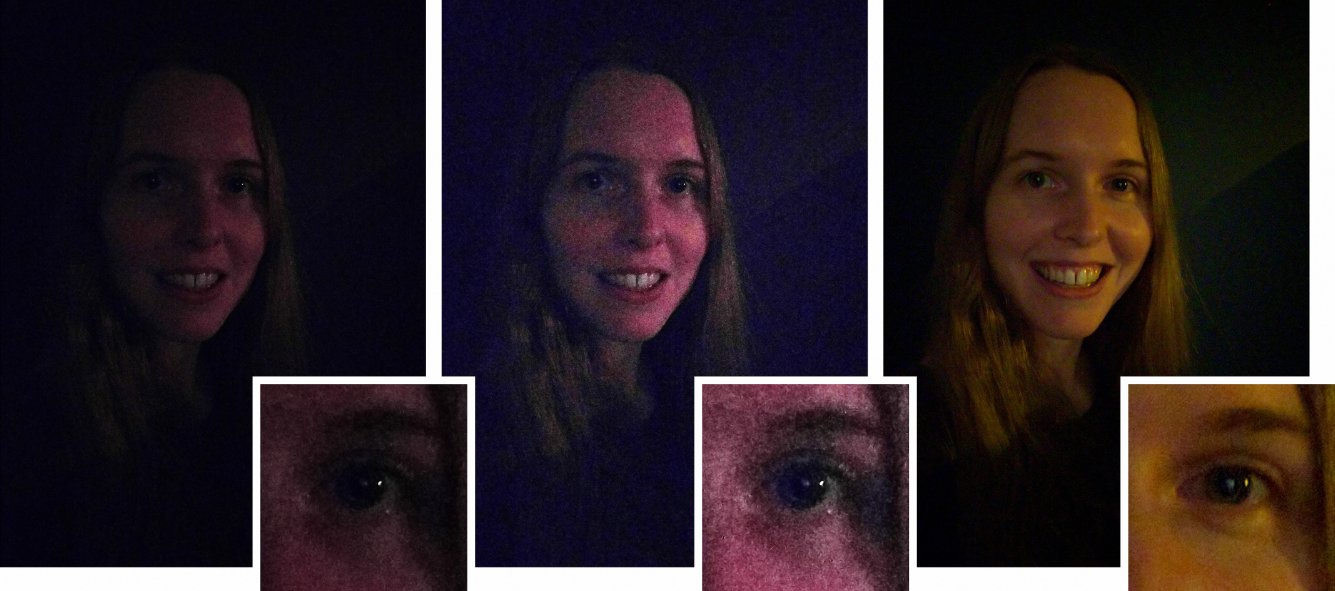
\includegraphics[width=0.70\textwidth]{figures/lowlight.png}
    \end{center}
    \caption{Burst photography comparison, left and middle captured with normal methods, right with burst photography~\cite{hasinoff2016burst}}\label{fig:lowlight}
\end{figure}

In this chapter we aim to give an overview of the computational photography
field itself, we cover some recent advancements in the field. How the
previously mentioned APIs have been used.

With the rise of fields like mobile phones, automotive, and robotics;
computational photography has become more important then ever. Due to size
constraints in many applications like mobile, the cameras themselves are often
not very good due to for example having a small aperture. To compensate this,
different IPAs have been developed. These IPAs allow for example the image to
look much brighter, clearer, or in general better.

Low light environments are difficult for mobile phones. In order for the camera
to compensate for this, one approach has been to increase gain, the issue is
that it simply generates noise. Another is to increase exposure, this can lead
to a blurry image due to shaking of the camera. A new approach has been to use
\textit{burst photography}~\cite{hasinoff2016burst} where a number of images
are captured. These images are then combined into a single image which allows
the algorithm to get a larger dynamic range than what would be possible with a
single image.

Additionally a concept called \textit{super resolution} has been developed, by
using artificial intelligence low resolution images can be scaled into high
resolution ones. There are a number of different approaches to this problem~\cite{yang2019deep, chen2022real}.
It is a difficult problem, especially \textit{singe image super resolution},
where only the one image is used.

In fields such as automotive we have begun seeing \textit{event cameras}~\cite{shariff2024event},
these are cameras that only report on pixels that "change"~\cite{rebecq2019events}.
Instead of receiving an entire frame at a time, the sensor would provide a
information that a single pixel  has changed. This allows the latency for
an image to be extremely low and very suitable for hard real time systems such
as cars. It is used to for example quickly detect pedestrians~\cite{wang2024research},
as normal sensors produce a lot of extra redundant data.
